% Standalone TikZ for Figure 4: SPI Transaction Timing & Arbiter Performance (clean, high color)
\documentclass[border=15pt]{standalone}
\usepackage{tikz}
\usetikzlibrary{positioning, arrows.meta, calc, decorations.pathreplacing, patterns, fit}
\definecolor{vbfcBlue}{HTML}{1B4F72}
\definecolor{vbfcDarkBlue}{HTML}{0D2B40}
\definecolor{vbfcAccent}{HTML}{E86C00}
\definecolor{vbfcLightGray}{HTML}{F2F2F2}
\definecolor{vbfcMediumGray}{HTML}{CCCCCC}
\definecolor{vbfcDarkGray}{HTML}{555555}
\definecolor{vbfcOrange}{HTML}{F39C12}
\definecolor{vbfcGreen}{HTML}{27AE60}
\definecolor{vbfcTeal}{HTML}{16A085}
\definecolor{vbfcPurple}{HTML}{8E44AD}
\definecolor{vbfcRed}{HTML}{C0392B}
\begin{document}
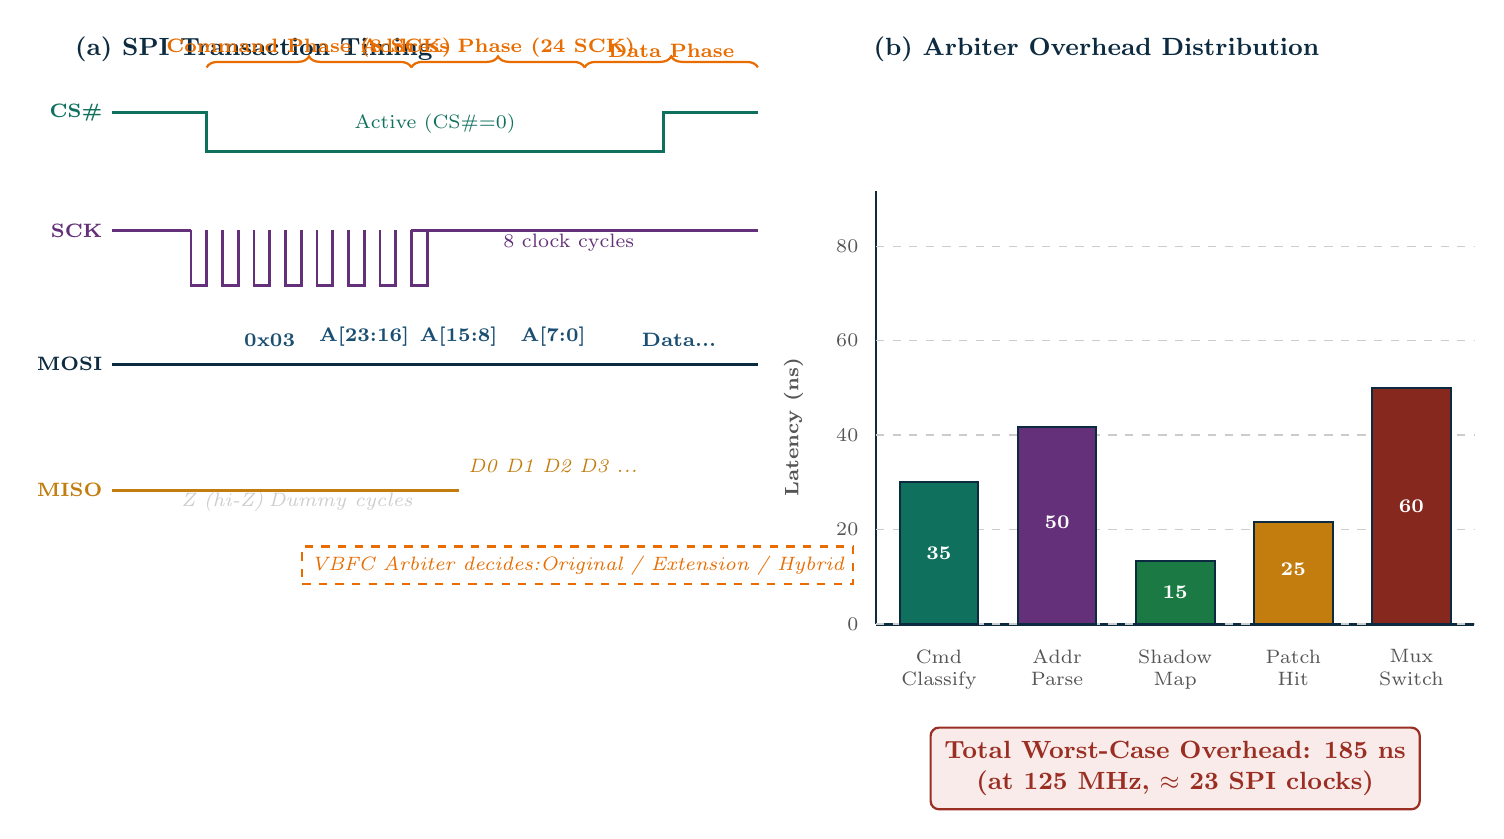
\begin{tikzpicture}[
    every node/.style={font=\scriptsize},
    axisline/.style={line width=1pt, draw=vbfcDarkBlue},
    gridline/.style={line width=0.5pt, draw=vbfcMediumGray, dashed},
    barlabel/.style={font=\scriptsize\bfseries, text=vbfcDarkBlue, anchor=center}
]

% ============================
% Left: Timing Diagram (original)
% ============================
% Title
\node[font=\small\bfseries, text=vbfcDarkBlue] at (18mm, 78mm) {(a) SPI Transaction Timing};

% CS# line (teal)
\node[anchor=east, font=\scriptsize\bfseries, text=vbfcTeal!70!black] at (0mm, 70mm) {CS\#};
\draw[axisline, draw=vbfcTeal!70!black] (0mm, 70mm) -- (12mm, 70mm) -- (12mm, 65mm) -- (70mm, 65mm) -- (70mm, 70mm) -- (82mm, 70mm);
\node[font=\scriptsize, text=vbfcTeal!70!black] at (41mm, 68.5mm) {Active (CS\#=0)};

% SCK line (purple)
\node[anchor=east, font=\scriptsize\bfseries, text=vbfcPurple!70!black] at (0mm, 55mm) {SCK};
\draw[axisline, draw=vbfcPurple!70!black] (0mm, 55mm) -- (10mm, 55mm);
\foreach \x in {10,14,18,22,26,30,34,38} {
    \pgfmathsetmacro{\xn}{\x+2}
    \draw[axisline, draw=vbfcPurple!70!black] (\x mm, 55mm) -- (\x mm, 48mm) -- (\xn mm, 48mm) -- (\xn mm, 55mm);
}
\draw[axisline, draw=vbfcPurple!70!black] (38mm, 55mm) -- (82mm, 55mm);
\node[font=\scriptsize, text=vbfcPurple!70!black] at (58mm, 53.5mm) {8 clock cycles};

% MOSI line (blue)
\node[anchor=east, font=\scriptsize\bfseries, text=vbfcDarkBlue] at (0mm, 38mm) {MOSI};
\draw[axisline] (0mm, 38mm) -- (82mm, 38mm);
\node[font=\scriptsize\bfseries, text=vbfcBlue, anchor=south] at (20mm, 39mm) {0x03};
\node[font=\scriptsize\bfseries, text=vbfcBlue, anchor=south] at (32mm, 39mm) {A[23:16]};
\node[font=\scriptsize\bfseries, text=vbfcBlue, anchor=south] at (44mm, 39mm) {A[15:8]};
\node[font=\scriptsize\bfseries, text=vbfcBlue, anchor=south] at (56mm, 39mm) {A[7:0]};
\node[font=\scriptsize\bfseries, text=vbfcBlue, anchor=south] at (72mm, 39mm) {Data...};

% MISO line (orange)
\node[anchor=east, font=\scriptsize\bfseries, text=vbfcOrange!80!black] at (0mm, 22mm) {MISO};
\draw[axisline, draw=vbfcOrange!80!black] (0mm, 22mm) -- (14mm, 22mm);
\node[font=\scriptsize\itshape, text=vbfcMediumGray] at (14mm, 20.5mm) {Z (hi-Z)};
\draw[axisline, draw=vbfcOrange!80!black] (14mm, 22mm) -- (44mm, 22mm);
\node[font=\scriptsize\itshape, text=vbfcOrange!80!black, anchor=south] at (56mm, 23mm) {D0 D1 D2 D3 ...};
\node[font=\scriptsize\itshape, text=vbfcMediumGray] at (29mm, 20.5mm) {Dummy cycles};

% Phase brackets
\draw[decorate, decoration={brace, amplitude=4pt, raise=2pt}, line width=0.8pt, draw=vbfcAccent]
    (12mm, 75mm) -- node[barlabel, text=vbfcAccent, anchor=south, yshift=2pt] {Command Phase (8 SCK)} (38mm, 75mm);
\draw[decorate, decoration={brace, amplitude=4pt, raise=2pt}, line width=0.8pt, draw=vbfcAccent]
    (38mm, 75mm) -- node[barlabel, text=vbfcAccent, anchor=south, yshift=2pt] {Address Phase (24 SCK)} (60mm, 75mm);
\draw[decorate, decoration={brace, amplitude=4pt, raise=2pt}, line width=0.8pt, draw=vbfcAccent]
    (60mm, 75mm) -- node[barlabel, text=vbfcAccent, anchor=south, yshift=2pt] {Data Phase} (82mm, 75mm);

% Arbiter acting
\node[draw=vbfcAccent, line width=0.8pt, dashed, font=\scriptsize\itshape, text=vbfcAccent, anchor=north west]
    at (24mm, 15mm) {VBFC Arbiter decides:\\Original / Extension / Hybrid};

% ============================
% Right: Bar chart (ARB latency overhead)
% ============================
% Title
\node[font=\small\bfseries, text=vbfcDarkBlue] at (125mm, 78mm) {(b) Arbiter Overhead Distribution};

% Bar chart axis
\draw[axisline] (97mm, 5mm) -- (173mm, 5mm);
\draw[axisline] (97mm, 5mm) -- (97mm, 60mm);

% Y axis ticks
\foreach \y/\lbl in {5/0, 17/20, 29/40, 41/60, 53/80} {
    \draw[gridline] (97mm, \y mm) -- (173mm, \y mm);
    \node[anchor=east, font=\scriptsize, text=vbfcDarkGray] at (96mm, \y mm) {\lbl};
}
\node[anchor=south, font=\scriptsize\bfseries, text=vbfcDarkGray, rotate=90] at (89mm, 30mm) {Latency (ns)};

% Bars
% Bar heights: Command classification = 35, Address parse = 50, Shadow map lookup = 15, Patch hit = 25, QSPI mux switch = 60
% CS for these operations
\filldraw[draw=vbfcDarkBlue, line width=0.7pt, fill=vbfcTeal!70!black]    (100mm, 5mm) rectangle (110mm, 23mm);
\node[barlabel, text=white] at (105mm, 14mm) {35};

\filldraw[draw=vbfcDarkBlue, line width=0.7pt, fill=vbfcPurple!70!black]  (115mm, 5mm) rectangle (125mm, 30mm);
\node[barlabel, text=white] at (120mm, 18mm) {50};

\filldraw[draw=vbfcDarkBlue, line width=0.7pt, fill=vbfcGreen!70!black]   (130mm, 5mm) rectangle (140mm, 13mm);
\node[barlabel, text=white] at (135mm, 9mm) {15};

\filldraw[draw=vbfcDarkBlue, line width=0.7pt, fill=vbfcOrange!80!black]  (145mm, 5mm) rectangle (155mm, 18mm);
\node[barlabel, text=white] at (150mm, 12mm) {25};

\filldraw[draw=vbfcDarkBlue, line width=0.7pt, fill=vbfcRed!70!black]     (160mm, 5mm) rectangle (170mm, 35mm);
\node[barlabel, text=white] at (165mm, 20mm) {60};

% X axis labels
\node[font=\scriptsize, text=vbfcDarkGray, anchor=north, align=center] at (105mm, 3mm) {Cmd\\Classify};
\node[font=\scriptsize, text=vbfcDarkGray, anchor=north, align=center] at (120mm, 3mm) {Addr\\Parse};
\node[font=\scriptsize, text=vbfcDarkGray, anchor=north, align=center] at (135mm, 3mm) {Shadow\\Map};
\node[font=\scriptsize, text=vbfcDarkGray, anchor=north, align=center] at (150mm, 3mm) {Patch\\Hit};
\node[font=\scriptsize, text=vbfcDarkGray, anchor=north, align=center] at (165mm, 3mm) {Mux\\Switch};

% Total overhead annotation
\node[draw=vbfcRed!80!black, line width=0.8pt, rounded corners=3pt, fill=vbfcRed!10,
      font=\small\bfseries, text=vbfcRed!80!black, anchor=north, inner sep=5pt, align=center]
      at (135mm, -8mm) {Total Worst-Case Overhead: \textbf{185 ns}\\(at 125 MHz, $\approx$ 23 SPI clocks)};

\end{tikzpicture}
\end{document}
